% The generic preamble
\documentclass[10pt,letterpaper,fleqn,titlepage]{article}

% Define packages to use
\usepackage{natbib}
\usepackage[dvips]{graphicx,color}
\usepackage{amsmath,amssymb}
\usepackage{bm}
\usepackage{caption}
\usepackage{xr}
\usepackage{ifthen}
\usepackage[dvipdfm,colorlinks,linkcolor=blue,citecolor=blue,urlcolor=blue]{hyperref}
\usepackage{fancybox}
\usepackage{textcomp}
\usepackage{alltt}
%\usepackage{floatflt}
%\usepackage{svn}


% Redefine default page
\setlength{\textheight}{9in}  % 1" above and below
\setlength{\textwidth}{6.75in}   % 0.5" left and right
\setlength{\oddsidemargin}{-0.25in}

% Redefine default paragraph
\setlength{\parindent}{0pt}
\setlength{\parskip}{1ex plus 0.5ex minus 0.2ex}

% Define caption width and default fonts
\setlength{\captionmargin}{0.5in}
\renewcommand{\captionfont}{\sffamily}
\renewcommand{\captionlabelfont}{\bfseries\sffamily}

% Define commands for super- and subscript in text mode
\newcommand{\superscript}[1]{\ensuremath{^\textrm{#1}}}
\newcommand{\subscript}[1]{\ensuremath{_\textrm{#1}}}

% Derived commands
\newcommand{\invcm}{\textrm{cm\superscript{-1}}}
\newcommand{\micron}{\ensuremath{\mu\textrm{m}}}

\newcommand{\df}{\ensuremath{\delta f}}
\newcommand{\Df}{\ensuremath{\Delta f}}
\newcommand{\dx}{\ensuremath{\delta x}}
\newcommand{\Dx}{\ensuremath{X_{max}}}
\newcommand{\Xeff}{\ensuremath{X_{eff}}}

\newcommand{\water}{\textrm{H\subscript{2}O}}
\newcommand{\carbondioxide}{\textrm{CO\subscript{2}}}
\newcommand{\ozone}{\textrm{O\subscript{3}}}

\newcommand{\taup}[1]{\ensuremath{\tau_{#1}}}
\newcommand{\efftaup}[1]{\ensuremath{\tau_{#1}^{*}}}

\newcommand{\textbfm}[1]{\boldmath\ensuremath{#1}\unboldmath}

\newcommand{\rb}[1]{\raisebox{1.5ex}[0pt]{#1}}

\newcommand{\f}[1]{\texttt{#1}}

% Define how equations are numbered
\numberwithin{equation}{section}
\numberwithin{figure}{section}
\numberwithin{table}{section}

% Define a command for title page author email footnote
\newcommand{\email}[1]
{%
  \renewcommand{\thefootnote}{\alph{footnote}}%
  \footnote{#1}
  \renewcommand{\thefootnote}{\arabic{footnote}}
}

% Define a command to print the Office Note subheading
\newcommand{\notesubheading}[1]
{%
  \ifthenelse{\equal{#1}{}}{}
  { {\Large\bfseries Office Note #1\par}%
    {\scriptsize \sc This is an unreviewed manuscript, primarily intended for informal}\\ 
    {\scriptsize \sc exchange of information among JCSDA researchers\par}%
  }
}

% Redefine the maketitle macro
\makeatletter
\def\docseries#1{\def\@docseries{#1}}
\def\docnumber#1{\def\@docnumber{#1}}
\renewcommand{\maketitle}
{%
  \thispagestyle{empty}
  \vspace*{1in}
  \begin{center}%
     \sffamily
     {\huge\bfseries Joint Center for Satellite Data Assimilation\par}%
     \notesubheading{\@docnumber}
  \end{center}
  \begin{flushleft}%
     \sffamily
     \vspace*{0.5in}
     {\Large\bfseries\ifthenelse{\equal{\@docseries}{}}{}{\@docseries: }\@title\par}%
     \medskip
     {\large\@author\par}%
     \medskip
     {\large\@date\par}%
     \bigskip\hrule\vspace*{2pc}%
  \end{flushleft}%
  \newpage
  \setcounter{footnote}{0}
}
\makeatother
\docseries{}
\docnumber{}


% Define a command for a DRAFT watermark
\usepackage{eso-pic}
\newcommand{\draftwatermark}
{
  \AddToShipoutPicture{%
    \definecolor{lightgray}{gray}{.85}
    \setlength{\unitlength}{1in}
    \put(2.5,3.5){%
      \rotatebox{45}{%
        \resizebox{4in}{1in}{%
          \textsf{\textcolor{lightgray}{DRAFT}}
        }
      }
    }
  }
}




% Title info
\title{Extra layering in the CRTM}
\author{Paul van Delst\email{paul.vandelst@noaa.gov}\\JCSDA/EMC/SAIC\\[0.25in]
        Yong Chen\email{yong.chen@noaa.gov}\\JCSDA/CIRA/STAR\\[0.25in]
        Yong Han\email{yong.han@noaa.gov}\\JCSDA/NESDIS/STAR}
\date{November, 2007}
\docnumber{(unassigned)}
\docseries{CRTM}


%-------------------------------------------------------------------------------
%                            Ze document begins...
%-------------------------------------------------------------------------------
\begin{document}
\maketitle

\begin{abstract}
The upper level temperature Jacobians produced by the CRTM can have apparently anomalous large values near the top of the atmosphere (TOA). Since the TOA is preset for the CompactOPTRAN algorithm, user input that does not extend that high is effectively extended in a thick layer to TOA in an isothermal manner for temperature, and constant mixing ratio for absorbers. To mitigate the impact of this thick top layer, extra layers of climatological profiles are added to the top of the user input profile in the CRTM. The methodology and results are discussed. It should be pointed out that this behaviour in the CRTM is not incorrect, but inherent to the CompactOPTRAN algorithm used 

\textbf{Keywords}: CRTM, CompactOPTRAN, temperature Jacobian, extra layering.
\end{abstract}



\section{Background}
%===================
\label{sec:background}
\subsection{Monochromatic transmittances}
%----------------------------------------
The monochromatic atmospheric transmittance, $\tau$, from some pressure level, $p$, to the top of the atmosphere (TOA) at some viewing angle, $\theta$, is given by,
\begin{equation}
  \tau(f,T,p,\theta) = \exp\left[-\left(\frac{\sec\theta}{g}\right)\sum_{j}\int_{p_{toa}}^{p}\chi_{j}(f,T,p') q_{j}(p')dp'\right]
  \label{eqn:tau}
\end{equation}
where $q_{j}(p)$ is the mass mixing ratio of molecular species $j$; $g$ is the acceleration due to gravity; and $\chi_{j}$ is the absorption coefficient of molecular species $j$ at frequency $f$, pressure $p$, and temperature $T(p)$. The OPTRAN algorithm\cite{OPTRAN3} recasts equation \ref{eqn:tau} in terms of the integrated absorber amount, $u$,
\begin{equation}
  u_{j}(p) = \frac{\sec\theta}{g}\int_{p_{toa}}^{p}q_{j}(p')dp'
  \label{eqn:int_u}
\end{equation}
using its differential form,
\begin{equation}
  du_{j} = \frac{\sec\theta}{g}q_{j}(p)dp
  \label{eqn:diff_u}
\end{equation}
Using equation \ref{eqn:diff_u} to perform variable substitution in equation \ref{eqn:tau}, we get,
\begin{equation}
  \tau(f,T,p,u) = \exp\left[-\sum_{j}\int_{u_{toa}}^{u_{j}}\chi_{j}(f,T(u_{j}'),p(u_{j}'))du_{j}'\right]
  \label{eqn:tau_u}
\end{equation}
Dropping the molecular species reference, $j$, for a given absorber we have\footnote{Equation \ref{eqn:tau_udu} is equivalent to equation(5) in \cite{OPTRAN3}},
\begin{equation}
  \tau(f,T,p,u+\Delta{u}) = \tau(f,T,p,u)\cdot\exp\left[-\int_{u}^{u+\Delta{u}}\chi(f,T(u'),p(u'))du'\right]
  \label{eqn:tau_udu}
\end{equation}
For a predefined set of discrete absorber amount levels, equation \ref{eqn:tau_udu} can be stated more concisely as the transmittance from \emph{level} $k$ to space,
\begin{equation}
  \tau_{k} = \tau_{k-1}\cdot\exp(-\chi_{k}\cdot\Delta{u}_{k})
  \label{eqn:simple_tau_udu}
\end{equation}
where both $\tau_{0}$ and $u_{0}$ are 0.0. Specifying layer optical depth, $\sigma_{k}$, as,
\begin{equation}
  \sigma_{k} = -\ln\left(\frac{\tau_{k}}{\tau_{k-1}}\right)
  \label{eqn:layer_od}
\end{equation}
we rearrange equation \ref{eqn:simple_tau_udu} to give an expression for the layer absorption coefficient in terms of the layer optical depth and absorber amount,
\begin{equation}
  \chi_{k} = \frac{\sigma_{k}}{\Delta{u}_{k}}
  \label{eqn:layer_chi}
\end{equation}


\subsection{Polychromatic transmittances}
%----------------------------------------
Up until now, we have been dealing with monochromatic transmittances at some frequency, $f$. Polychromatic, instrument resolution transmittances are obtained by convolving the monochromatic transmittances with a spectral response function (SRF), $\phi(f)$
\begin{equation}
  \tau_{k}(\Delta{f}) = \int_{\Delta{f}}\tau_{k}(f)\phi(f)df
  \label{eqn:poly_tau}
\end{equation}
Assigning the subscript $l$ to a particular sensor channel $\phi(f)$ integration, the monochromatic equations \ref{eqn:simple_tau_udu} to \ref{eqn:layer_chi} are here simply recast in terms of polychromatic transmittances for use in a regression equation with $I$ predictors to give,
\begin{equation}
  \chi_{k,l} = \sum_{i}^{I}b_{i,k,l}\cdot X_{i,k}
  \label{eqn:reg_layer_chi}
\end{equation}
where the $b$ are the regression coefficients and $X$ are the predictors. It was found\cite{OPTRAN1}\cite{OPTRAN3} that to preserve accuracy in the resultant polychromatic transmittances scaling approximations were required to be used. Thus, some of the predictors in \ref{eqn:reg_layer_chi} are absorber averaged temperature and pressures of the form,
\begin{eqnarray}
  T_{k}^{*(n)} & = & \frac{\displaystyle\int_{u_{toa}}^{u_{k}}u^{n-1}T(u)du}{\displaystyle\int_{0}^{u_{k}}u^{n-1}du}\nonumber\\
  \textrm{and} & &\\
  p_{k}^{*(n)} & = & \frac{\displaystyle\int_{u_{toa}}^{u_{k}}u^{n-1}p(u)du}{\displaystyle\int_{0}^{u_{k}}u^{n-1}du}\nonumber
\end{eqnarray}
A full description of the origin of these predictors is more nuanced and can be found in \cite{OPTRAN3}. The important thing to note here (and in equation \ref{eqn:tau_u}) is the lower integration limit, $u_{toa}$.

Note that the polychromatic optical depths and absorption coefficients derived from the result of equation \ref{eqn:poly_tau} used in equations \ref{eqn:layer_od} and \ref{eqn:layer_chi} are inherently non-physical.


\subsection{The CompactOPTRAN algorithm}
%---------------------------------------
\label{sec:compact_optran}
The CompactOPTRAN absorption algorithm computes an integrated absorber space level associated with the average layer absorber amount for three different absorbers: water vapour, ozone, and the dry (or fixed) gases. For the dry gas absorbers, pressure is used as a proxy absorber amount. This means the start of the dry gas absorber space is always at the defined TOA pressure of the dependent set profiles used in the regression, i.e. 0.005hPa.

Conversion of an absorber level, $k$, to an average layer absorber amount, $\bar{u}$, is given by,
\begin{equation}
  \bar{u}_{k} = c_{1}\cdot\exp(\alpha\cdot k) + c_{2}
\end{equation}
with the inverse given by,
\begin{equation}
  k = \frac{1}{\alpha}\cdot\ln\left(\frac{\bar{u}(k) - c_{2}}{c_{1}}\right)
\end{equation}
where $\alpha$ is a constant for converting from absorber amount to level coordinate, and $c_{1}$ and $c_{2}$ are scaling factors to ensure the level value, $k$, remains in the range 0 to 1.

For every atmospheric predictor, $X_{i}$, the regression coefficient associated with it for a particular channel, $l$, at a particular absorber amount level, $k$, is given by an $N^{th}$ order polynomial,
\begin{equation}
  b_{i,k,l} = \sum_{n=0}^{N} c_{n,i,l}\cdot k^{n}
\end{equation}
The logarithm of the absorption coefficient, $\chi$, is then determined from the regression equation,
\begin{equation}
  \ln(\chi_{k,l}) = b_{0,k,l} + \sum_{i=1}^{I} b_{i,k,l}\cdot X_{i}
\end{equation}
and the layer optical depth, $\sigma$, is then given by,
\begin{equation}
  \sigma_{k,l} = \chi_{k,l}\cdot\Delta{u_{k}}
\end{equation}


\section{The issue}
%==================
As described in section \ref{sec:background} the CompactOPTRAN absorption algorithm that is currently used in the CRTM operates in absorber, rather than pressure, level space. That is, regression coefficients to compute atmospheric absorption are associated with specific integrated absorber amounts rather than pressure levels\footnote{Other fast transmittance models, like that used in RTTOV, operate on fixed pressure levels}. 

The CompactOPTRAN absorption algorithm computes an integrated absorber space level associated with the average layer absorber amount for three different absorbers: water vapour, ozone, and the dry (or fixed) gases. For the dry gas absorbers, pressure is used as a proxy absorber amount. This means that, unlike the water vapour and ozone absorbers, the start of the dry gas absorber space is always at the defined TOA pressure of the dependent set profiles used in the regression, i.e. 0.005hPa.

User atmospheric profile input to the CRTM rarely extend to 0.005hPa. As such, the CompactOPTRAN algorithm treats the atmosphere from the bottom of the first user input level to its default TOA as a single layer. The consequence of this is that the top layer used in the CRTM can be very thick. For water vapour and ozone Jacobians this is not an issue since the absorber spaces will always start at 0.0 regardless of what pressure level the input profile begins at. However, since the temperature Jacobians mostly involve absorption by the dry gas absorbers (in particular \carbondioxide) the top layer computed Jacobians are correspondingly large compared with those of the layers directly below because the regression coefficients always begin at 0.005hPa.

To prevent these large excursions in the top layer temperature Jacobians, the user input atmospheric profile is supplemented with climatological profile data up to the CRTM default TOA of 0.005hPa. It should be noted that this addition of extra profile layers may not be applicable to NWP applications since, while the top average \emph{layer} pressure of an input atmospheric profile may be well below 0.005hPa, the top pressure \emph{level} may not.


\section{Supplementing the input profile}
%========================================
For simplicity, the approach adopted was to simply copy the user input atmospheric profile and supplement that copy with climatolgical data. This supplemented profile is then passed through the usual CRTM call chain. For cloudy profiles this could be computational expensive since if clouds are present anywhere in the profile, the CRTM ADA radiative transfer (RT) solver is used for the entire atmospheric column. Since there is no cloud information in the supplemental climatology data used, there is no need to perform cloudy radiative transfer in that part of the column. This issue, however, will be dealt with in future updates to the RT code.


\subsection{Selecting the climatology}
%-------------------------------------
The user selects the climatolgy used for supplementing the input profile by setting the \texttt{Climatology} component in the \texttt{CRTM\_Atmosphere} structure. The available climatological profiles are shown in table \ref{tab:climatology}. The parameter definitions are available when the main CRTM module is used via the \texttt{USE} statement, for example:
\begin{verbatim}
  USE CRTM_Module
  ...
  TYPE(CRTM_Atmsophere_type) :: Atm(1)
  ...
  Atm(1)%Climatology = MIDLATITUDE_WINTER
\end{verbatim}
Invalid definitions default to the U.S. Standard Atmosphere.
\begin{table}[htp]
  \centering
  \begin{tabular}{c | c}
    Climatology Model & Parameter Name\\
    \hline
    Tropical                 & \texttt{TROPICAL}\\
    Midlatitude summer       & \texttt{MIDLATITUDE\_SUMMER}\\
    Midlatitude winter       & \texttt{MIDLATITUDE\_WINTER}\\
    Subarctic summer         & \texttt{SUBARCTIC\_SUMMER}\\
    Subarctic winter         & \texttt{SUBARCTIC\_WINTER}\\
    U.S. Standard Atmosphere & \texttt{US\_STANDARD\_ATMOSPHERE}
  \end{tabular}
  \caption{CRTM Atmosphere structure Climatology valid values.}
  \label{tab:climatology}
\end{table}


\subsection{Blending the climatology profile with user data}
%-----------------------------------------------------------
To minimise discontinuities in profiles that have climatological model data added at TOA, the added data must be ``blended'' with the user input. The procedure used is shown schematically in figure \ref{fig:blend_profile}
\begin{figure}[htp]
  \centering
  \includegraphics[scale=0.8]{graphics/blend_profile.eps}
  \caption{Schematic of user and model profile blending methodology. Black: User profile; Red: Model profile; Blue: Interpolated values; Green: Shifted model profile.}
  \label{fig:blend_profile}
\end{figure}
The model profile is interpolated to the top user profile pressure, $P_{u}(0)$, yielding the quantity $X_{m,int}\left(P_{u}(0)\right)$ (where here $X$ refers to any of the profile quantities in question: temperature, water vapour mixing ratio, or ozone mixing ratio). The first layer model average is,
\begin{equation*}
  \bar{X}_{m}\left(N\right) = \frac{X_{m,int}\left(P_{u}(0)\right) + X_{m}\left(N-1\right)}{2}
\end{equation*}
Given that,
\begin{equation*}
  \bar{P}_{u,m}\left(N\right) = \frac{P_{u}\left(0\right) - P_{m}\left(N-1\right)}{\ln{}\bigg(\frac{\displaystyle P_{u}\left(0\right)}{\displaystyle P_{m}\left(N-1\right)}\bigg)}
\end{equation*}
then the user profile ``layer 0'' value can be approximated by linearly extrapolating in $\ln{(P)}$ the top \emph{layer} user values. The interpolating polynomial is given by,
\begin{equation*}
  lp_{0} = \frac{\ln\left(\bar{P}_{u,m}\left(N\right)\right) - \ln\left(\bar{P}_{u}\left(1\right)\right)}
                {\ln\left(\bar{P}_{u}  \left(2\right)\right) - \ln\left(\bar{P}_{u}\left(1\right)\right)}
\end{equation*}
with the extrapolated value being,
\begin{equation*}
  \bar{X}_{u}(0) = \left(\bar{X}_{u}(2) - \bar{X}_{u}(1)\right)\cdot lp_{0} + \bar{X}_{u}(1)
\end{equation*}
The difference between this ``layer 0'' value and the first layer model average,
\begin{equation*}
  \Delta X = \bar{X}_{u}(0) - \bar{X}_{m}(N)
\end{equation*}
is then used to shift the model \emph{level} profile so there is no discontinuity at $\bar{P}_{u,m}\left(N\right)$,
\begin{equation*}
  X_{m} = X_{m} + \Delta X
\end{equation*}
These shifted level values are then averaged to produce the final blended profile. This is done for the water vapour and ozone absorber amounts also, but with a check for negative values. An example of a supplemented profile showing the unshifted and shifted model data is shown in figure \ref{fig:blended_profile49} for a profile from the ECMWF set of 52 model profiles\cite{ECMWF_profile_set}\footnote{Profiles were interpolated to the standard 101-levels used for AIRS processing}.
\begin{figure}[htp]
  \centering
  \includegraphics[scale=0.8]{graphics/ECMWF.blended_profile_49.eps}
  \caption{An example of the profile extension showing the shift applied to the data to minimise discontinuities across the user and model profile boundary. ECMWF profile 49.}
  \label{fig:blended_profile49}
\end{figure}


\section{Impact of extra layering}
%=================================
With reference to section \ref{sec:background}, and section \ref{sec:compact_optran} in particular, modifying the absorber space by supplementing additional layers at TOA can modify the computed absorber level, $k$, which can produce slightly different regression coefficients, $b_{i,k,l}$, which in turn can produce slightly different absorption coefficients and optical depths.

All of the brightness temperature differences shown in this section are for profile 1 of the ECMWF set, the truncated and supplemented versions of which are shown in figure \ref{fig:blended_profile01}. Calculations were done for a standard set of instruments: NOAA-18 HIRS/4, AMSU-A, and MHS; and Aqua AIRS.
\begin{figure}[htp]
  \centering
  \includegraphics[scale=0.8]{graphics/ECMWF.blended_profile_01.eps}
  \caption{Truncated and supplemented atmospheric profiles for ECMWF profile 1 used to generate the brightness temperatures differences shown in this section.}
  \label{fig:blended_profile01}
\end{figure}


\subsection{Forward model}
%-------------------------
The impact of supplementing the upper layers of an input user profile in the CRTM forward model is shown in figures \ref{fig:hirs4_n18.fwd_el.p1}, \ref{fig:amsua_n18.fwd_el.p1}, and \ref{fig:airs_aqua.fwd_el.p1} for the NOAA-18 HIRS/4, NOAA-18 AMSU-A, and Aqua AIRS respectively. As expected, the largest differences occur for those channels that are sensitive to absorption in the upper atmosphere.
\begin{figure}[htp]
  \centering
  \includegraphics[scale=0.8]{graphics/hirs4_n18.fwd_el.p1.eps}
  \caption{Impact of the extra layering on NOAA-18 HIRS brightness temperatures. ECMWF profile 1.}
  \label{fig:hirs4_n18.fwd_el.p1}
\end{figure}
\begin{figure}[htp]
  \centering
  \includegraphics[scale=0.8]{graphics/amsua_n18.fwd_el.p1.eps}
  \caption{Impact of the extra layering on NOAA-18 AMSU-A brightness temperatures. ECMWF profile 1.}
  \label{fig:amsua_n18.fwd_el.p1}
\end{figure}
\begin{figure}[htp]
  \centering
  \includegraphics[scale=0.8]{graphics/airs_aqua.fwd_el.p1.eps}
  \caption{Impact of the extra layering on Aqua AIRS brightness temperatures. ECMWF profile 1.}
  \label{fig:airs_aqua.fwd_el.p1}
\end{figure}


\subsection{K-Matrix model}
%--------------------------

\subsubsection{Temperature Jacobians}
%....................................
The impact of supplementing the upper layers of an input user profile in the CRTM K-matrix model is shown in the temperature Jacobians of figures \ref{fig:hirs4_n18.t_k_el.p1}, \ref{fig:amsua_n18.t_k_el.p1}, and \ref{fig:airs_aqua.t_k_el.p1} for the NOAA-18 HIRS/4, NOAA-18 AMSU-A, and Aqua AIRS (selected channels only) respectively. The top layer or two of the temperature Jacobians without the extra layering clearly show the anomaly at TOA. Adding the extra profile layers removes this problem.

An additional effect of the TOA extra layering is that the differences in the temperature Jacobians are not contained to the top few layers of the atmosphere. Some of the channel Jacobians, particularly for the infrared instruments, show significant differences at lower levels when the profiles are supplemented. In particular, AIRS channel 216 ($f_{0}$=711.293\invcm) in figure \ref{fig:airs_aqua.t_k_el.p1} stands out with a relative difference of ~27\% centred at approximately 350hPa. The Jacobian differences for some of the HIRS channels in figure \ref{fig:hirs4_n18.t_k_el.p1} also occur at lower levels in the atmosphere, but the magnitude of those difference is much smaller.

\begin{figure}[htp]
  \centering
  \includegraphics[scale=0.8]{graphics/hirs4_n18.t_k_el.p1.eps}
  \caption{Impact of the extra layering on NOAA-18 HIRS temperature Jacobians. ECMWF profile 1.}
  \label{fig:hirs4_n18.t_k_el.p1}
\end{figure}
\begin{figure}[htp]
  \centering
  \includegraphics[scale=0.8]{graphics/amsua_n18.t_k_el.p1.eps}
  \caption{Impact of the extra layering on NOAA-18 AMSU-A temperature Jacobians. ECMWF profile 1.}
  \label{fig:amsua_n18.t_k_el.p1}
\end{figure}
\begin{figure}[htp]
  \centering
  \includegraphics[scale=0.8]{graphics/airs_aqua.t_k_el.p1.eps}
  \caption{Impact of the extra layering on Aqua AIRS temperature Jacobians for selected channels in the 15\micron{} \carbondioxide{} band. ECMWF profile 1. $f_{0}$(ch22)=654.659\invcm, $f_{0}$(ch321)=742.227\invcm }
  \label{fig:airs_aqua.t_k_el.p1}
\end{figure}


\subsubsection{Water Vapour Jacobians}
%.....................................
The impact of the TOA extra layering on the water vapour Jacobians is smaller than for the temperature Jacobians. The changes in the NOAA-18 HIRS/4, AMSU-A, and MHS water vapour Jacobians for ECMWF profile 1 are shown in figures \ref{fig:hirs4_n18.h2o_k_el.p1}, \ref{fig:amsua_n18.h2o_k_el.p1}, and \ref{fig:mhs_n18.h2o_k_el.p1} respectively; and the change for selected AIRS water vapour channels is shown in figure \ref{fig:airs_aqua.h2o_k_el.p1}. The differences between the Jacobians are generally several orders of magnitude less than the Jacobian value itself but, as with the temperature Jacobians, the differences occur throughout the atmospheric column.
\begin{figure}[htp]
  \centering
  \includegraphics[scale=0.8]{graphics/hirs4_n18.h2o_k_el.p1.eps}
  \caption{Impact of the extra layering on NOAA-18 HIRS water vapour Jacobians. ECMWF profile 1.}
  \label{fig:hirs4_n18.h2o_k_el.p1}
\end{figure}
\begin{figure}[htp]
  \centering
  \includegraphics[scale=0.8]{graphics/amsua_n18.h2o_k_el.p1.eps}
  \caption{Impact of the extra layering on NOAA-18 AMSU-A water vapour Jacobians. ECMWF profile 1.}
  \label{fig:amsua_n18.h2o_k_el.p1}
\end{figure}
\begin{figure}[htp]
  \centering
  \includegraphics[scale=0.8]{graphics/mhs_n18.h2o_k_el.p1.eps}
  \caption{Impact of the extra layering on NOAA-18 MHS water vapour Jacobians. ECMWF profile 1.}
  \label{fig:mhs_n18.h2o_k_el.p1}
\end{figure}
\begin{figure}[htp]
  \centering
  \includegraphics[scale=0.8]{graphics/airs_aqua.h2o_k_el.p1.eps}
  \caption{Impact of the extra layering on Aqua AIRS water vapour Jacobians for selected channels in the 6.7\micron{} \water{} band. ECMWF profile 1. $f_{0}$(ch1500)=1357.236\invcm, $f_{0}$(ch1620)=1423.179\invcm }
  \label{fig:airs_aqua.h2o_k_el.p1}
\end{figure}


\subsubsection{Ozone Jacobians}
%..............................
The impact of the TOA extra layering on the ozone Jacobians from the infrared instruments is also much smaller than for the temperature Jacobians. The changes in the NOAA-18 HIRS/4 and selected Aqua AIRS ozone channel Jacobians for ECMWF profile 1 are shown in figures \ref{fig:hirs4_n18.o3_k_el.p1} and \ref{fig:airs_aqua.o3_k_el.p1} respectively. The character of the differences is similar to that for the water vapour Jacobian differences: generally several orders of magnitude less than the Jacobian value itself but spread throughout the atmospheric column.
\begin{figure}[htp]
  \centering
  \includegraphics[scale=0.8]{graphics/hirs4_n18.o3_k_el.p1.eps}
  \caption{Impact of the extra layering on NOAA-18 HIRS ozone Jacobians. ECMWF profile 1.}
  \label{fig:hirs4_n18.o3_k_el.p1}
\end{figure}
\begin{figure}[htp]
  \centering
  \includegraphics[scale=0.8]{graphics/airs_aqua.o3_k_el.p1.eps}
  \caption{Impact of the extra layering on Aqua AIRS ozone Jacobians for selected channels in the 9.7\micron{} \ozone{} band. ECMWF profile 1. $f_{0}$(ch1000)=1000.098\invcm, $f_{0}$(ch1120)=1063.767\invcm }
  \label{fig:airs_aqua.o3_k_el.p1}
\end{figure}


% The references section
%=======================
\bibliographystyle{plain}
\bibliography{bibliography}	


% The appendices section
%=======================
%\begin{appendix}
%\end{appendix}


\end{document}

